\section{The Cosmological Context of Galaxy Formation}
The modern picture of galaxy formation sits within the context of a $\Lambda$
Cold Dark Matter  ($\Lambda CDM$) cosmology \citet{White1978,Mo1998}.  This is a
universe which has a no curvature ($\Omega = 1$), and today has the majority of
its mass-energy in a cosmological constant $\Lambda$ ($\Omega_\Lambda \sim
0.7$), and most of its matter in a collisionless form (Dark matter) ($\Omega_m
\sim 0.3$) \citep{Planck2014}.  Roughly $5\%$ of the universe exists as baryons ($\Omega_b \sim
0.05$), which began as a mostly isothermal gas of hydrogen and helium.  All of
this began roughly $13.8$ billion years ago, with the universe emerging from a
state of infinite temperature and density, expanding to form what we see today.
The primordial elemental abundances, with $\sim4/5$ of the universe's baryons in
hydrogen, and the remainder in helium, was established just a few minutes after
the big bang, during a brief period of ``Big Bang Nucleosynthesis''
\citep{Alpher1948}.  The remaining elements of the periodic table have been
formed through stellar nucleosynthesis, through fusion in the cores of stars and
in energetic processes that take place during supernovae (SN)\citet{Wagoner1967}.

Much of what we know about the cosmology of our universe comes from observations
of the first light to escape the universe as it became optically thin: the
cosmic microwave background (CMB).  Prior to a redshift of $z=1100$, the
universe had a high ionization fraction such that the mean free path for
photons was short, making all of space effectively opaque.  Once the universe
became cool enough that hydrogen became neutral, the optical depth was now low
enough that photons could free-stream, decoupled from baryons.  This ultraviolet
light we observe today, redshifted to microwaves with a temperature just
$\sim2.7\;\rm{K}$.  When the power spectrum of this radiation is measured,
features in that spectrum can be used to determine the components of the
universe, as well as the spectrum of density perturbations that will eventually
form galaxies.

The formation of galaxies within the universe began with the gravitational
collapse of small, linear density perturbations that were likely seeded by
quantum fluctuations amplified by inflation.  These perturbations grow through
gravitational collapse.  Until $z\sim1100$, only dark matter perturbations were
able to grow.  Prior to this, baryons were coupled to photons, causing density
perturbations to simply oscillate as stable sound waves.  This early collapse of
matter meant that when decoupling occurred at $z\sim1100$, baryons were able to
collapse into the deeper potential wells grown out of dark-matter density
perturbations.  These overdensities expand slower that the surrounding medium,
as they experience a drag from their own self-gravity.  Eventually, these
regions stop expanding altogether and begin collapsing at the turnaround time
$t_{turn}$, and virialize at $2t_{turn}$. The first galaxies likely began to
form around $z\sim20-50$.

The perturbation spectrum that forms the structure in which galaxies begins to
form is essentially a Gaussian random field, which \citet{Press1974} were able
to show produces a halo mass spectrum at a given time with a relatively simple form:
\begin{equation}
    \frac{dn}{dM}(M,t) =
    \sqrt{\frac{2}{\pi}}\frac{\rho_0\delta_c(t)}{M^2\sigma(M)} 
    \left\lvert\frac{d\ln{\sigma}}{d\ln{M}}\right\rvert
    \exp{\left[-\frac{\delta^2_c(t)}{2\sigma^2(M)}\right]}
\end{equation}
In this equation, $\rho_0$ is the mean density of the universe, and
$\delta_c(t)$ is the critical overdensity for collapse at a given time $t$.  The
mass variance spectrum, $\sigma^2(M)$ can be determined observationally using
the CMB power spectrum \citep{Planck2015}.  This function gives a distribution
of masses for the dark matter halos that galaxies will begin to form within.  As
these halos collapse, gravitational torques from their surroundings will impart
torques on them \citep{Barnes1987}, causing galaxies to have a distribution of angular momenta.
High resolution N-body simulations have found that dark matter halos have both a
universal density profile \citep{Navarro1996,Merritt2006} as well as a universal
angular momentum profile \citep{Bullock2001}.  

The collapse of baryons within the will depend strongly on whether the
post-virialized gas can cool radiatively \citep{Rees1977}.  As gas accretes onto
a halo with overdensity $\Delta$ it passes through a shock that raises its
temperature to the virial temperature:
\begin{equation}
    T_{virial} = \frac{2}{3}\frac{G\mu m_H}{k_B}\left({\frac{4\pi\rho_0\Delta
    M^2}{3}}\right)^{1/3}
\end{equation}
This means that more massive halos have larger virial temperatures, and,
depending on the mode of radiative cooling (atomic cooling from primordial
hydrogen, molecular hydrogen cooling, or cooling through metal lines), this may
give cooling times shorter than the current age of the universe.  These halos 
are the ones in which galaxy formation may begin, as their hot gaseous halos may
can collapse to form a disk, with a cold ISM where star formation can occur.

As gas does begin to cool within these halos, it will lose pressure support (by
radiating away thermal energy), but {\it not} angular momentum.  This means that
the baryons, which typically carry the same specific angular momentum as the
halo itself, will flatten to form an exponential disc as they cool
\citep{Fall1980,Mo1998}.  Within this disc, an interstellar medium (ISM) will form.  This
ISM is multiphase, containing both hot ($T\sim10^5\;\rm{K}$) and cold
($T\sim10-100\;\rm{K}$) in quasistatic equilibrium \citep{McKee1977}.
\begin{figure}
    \includegraphics[width=0.7\textwidth]{mass_function.eps}
    \caption[Galaxy mass function]{The observed mass function for galaxies in
    the nearby universe does not match the mass function for dark matter halos
    given in equation 1, scaled by the baryon fraction.  This tells us that
    there are additional physical processes involved in the formation of
    galaxies within their dark matter halos.  The most likely candidate for
    this is feedback from stars and black holes.  Of particular interest is the
    peak in star formation efficiency near $M_{200}=10^{12}M_\odot$.
    \textit{Image credit: Adapted from figure 1 in \citet{Ferrero2012}}}.
\end{figure}

This is of course all highly idealized, simple models for the earliest stages
and broadest strokes of galaxy formation.  Each of these halos will begin to
undergo mergers and interactions with each other that can strip stars and gas
through tidal and ram pressure forces.  Inside each of these halos, the process
of disc collapse, the formation of a multiphase ISM, star
formation, and feedback from those stars involves the complex, nonlinear
interplay of radiation, hydrodynamics, magnetic fields, and gravity on length
scales as much as $10^{11}$ times smaller than the virial radius.  None of this
physics is simple enough to be captured by these sorts of analytic models, and
so numerical simulations have become a keystone for galaxy formation research.

Numerical modeling of galaxies is a difficult problem, as it involves processes
that take place over scales (both spatial and temporal) that span many orders of
magnitude.  This means that simulations will always be unable to resolve at
least some fraction of the physics taking place within the galaxy.  For this,
carefully designed ``sub-grid'' models are required to include the macroscopic
effects that unresolvable microscopic processes yield. 

\section{Numerical Simulations of Galaxies}
Simulations of galaxies actually predate {\it numerical} simulations of
galaxies.  \citet{Holmberg1941} presented, as the author termed it, a ``new
integration procedure'' that was arguably the first attempt to simulate the
evolution of galaxy.  By relying on the fact that light flux, just as gravity,
scales as $r^{-2}$, Holmberg was able to construct a simulated galaxy disc out
of light bulbs, and then using photocells to measure the flux at each bulb's
position, repositioned the bulbs using the forces ``simulated'' by the
light-measuring process.  This allowed him to painstakingly trace the tidal
interactions of passing galaxies as they fell into a galaxy cluster.

In the intervening 75 years, we have migrated to much less labor-intensive
simulations, relying on the constantly growing power of digital computers.  As
Gordon Moore first observed in 1965, the processing power of computers has been
continuously growing at an exponential rate for more than half a century.  This
has meant that, even without advances in numerical methods and algorithm design,
the ability of simulators today to model a system in high resolution is
monumentally greater than just 10 years ago.  

\begin{figure}
    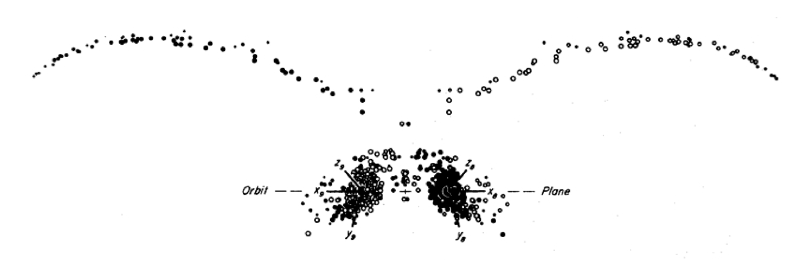
\includegraphics[width=0.8\textwidth]{Toomre.eps}
    \includegraphics[width=0.8\textwidth]{Antennae.eps}
    \caption[Early simulation of Antennae Galaxies]{The simulations of
    \citet{Toomre1972} showed how the kinematics of galaxy mergers can produce
    the variety of tidal structures seen in objects like the Antennae galaxies.
    The top image shows the result of one of the \citet{Toomre1972} simulations.
    \textit{Image credit: Adapted from figure 23 of \citet{Toomre1972}}
    The bottom image shows an observation of the actual object itself, the
    Antennae galaxies NGC 4038/4039. \textit{Image credit: NOAO/AURA/NSF, B.
    Twardy, B. Twardy, and A. Block (NOAO)}}
\end{figure}

The earliest numerical simulations of galaxy formation focused on the
effects of gravity alone.  A classic example of this are the simulations
presented in \citet{Toomre1972}, which showed that the irregular structures seen
in galaxies like NGC 4676 (``The Mice'') or NGC4038/4039 (``The Antennae
Galaxies'') are the results of major mergers between two disc galaxies.  These
simulations used discs composed of a mere 120 test particles, and ignored the
effects of self-gravity between these particles.  Despite the crudeness of these
simulations, these simulations definitively showed that galactic bridges and
tails could be formed by the tidal interactions of two passing/merging galaxies.
The IBM 360/95 that \citet{Toomre1972} (with an inflation-adjusted purchase
price in the millions of dollars) used for their simulations was capable of
5.5 million instructions per second, roughly $0.2\%$ the speed of the 35\$
Raspberry Pi 3 available today.

Modern galaxy simulations do far more than merely integrate the equations of
motion for a few hundred test particles in a gravitational field.  Today, state
of the art simulations will track gravity (including self-gravity) for stars,
gas, and dark matter; evolve Euler's equations for the hydrodynamics of gaseous
baryons; include models for radiative cooling of gas that allow for cooling from
both hydrogen and metal lines; form stars from dense gas; and include models for
feedback from massive stars and black holes.  Often, simulations will also
include treatments for radiative transfer and magneto-hydrodynamics as well.

Gravity is typically solved using algorithms designed to minimize the workload
that would be needed for a direct summation of each particle or grid cell
($\mathcal{O}(N^2)$ for N grid cells/particles).  This becomes intractable for
larger numbers of resolution elements, as the workload will scale as the sixth
power of the linear resolution (an order of magnitude better linear resolution
will be $10^6$ times more expensive!).  In order to reduce these costs,
algorithms have been developed that allow for more efficient gravitational
force calculations.  Tree-based methods \citep{Barnes1986} reduce the
computational cost of long-ranged (and thus less significant) force
calculations by using space-partitioning trees.  Short-range force calculations
are done particle-by-particle, while long-range forces are calculated against
larger tree cells, thus reducing the cost of calculating gravity to
$\mathcal{O}(N\log N)$.  Particle-Particle/Particle-Mesh ($P^3M$) methods
\citep{Couchman1991} take a produce similar scalings, but rather than using a
spatial tree rely on a spectral Fourier-based approach to calculate long-ranged
interactions.  Recently, the Fast Multipole Method \citep{Greengard1987} has
been adapted for calculation of gravitational forces
\citep{Dehnen2002,Hahn2013} using a multipole expansion of Green's functions.
This allows for extremely efficient gravity calculation, scaling linearly with
particle number ($\mathcal{O}(N)$).

Hydrodynamical solvers usually come in one of two classes: Eulerian or
Lagrangian.  Eulerian methods discretize space, breaking a simulation volume
into a grid of cells that each contains a number of scalar and vector
quantities that are advected according to the solver scheme.  Eulerian schemes
typically allow for higher-order solvers, lower intrinsic noise, and better
resolved discontinuities \citep{Teyssier2002,Stone2008,Bryan2014}.  They suffer
from intrinsic mixing and diffusion that scales with the flow velocity relative
to the grid \citet{Agertz2007,Tasker2008}.  Lagrangian methods instead
discretize mass, breaking the gaseous volume into discrete points, each of
which is moved to advect the quantities it contains, with smoothing functions
used to interpolate values in between particles.  Lagrangian methods couple
easily to tree codes for gravity calculation, are Galilean invariant, and
intrinsically conserve mass, energy, and momentum (linear and angular)
\citep{Katz1996,Wadsley2004,Springel2005}.  They require the use of artificial
viscosity to handle shocks, and as such have difficulty in capturing subsonic
turbulence \citep{Bauer2012}. Recently, new methods have begin to hybridize
features of each of these classes as well \citep{Springel2010,Hopkins2015}. 

Modern galaxy simulations also now use a variety of strategies for judiciously
applying computational power where it is most needed.  Eulerian methods will
commonly use \textit{Adaptive Mesh Refinement} to increase resolution in regions of
interest (typically where gas is densest).  Lagrangian methods automatically do
this, as a denser region definitionally must contain more particles.  Beyond the
choice of algorithms, the choice of what type of simulation to set up in the
initial conditions is also important.  To study large populations of galaxies,
along with large-scale structure, large-volume cosmological boxes with
$>>10^4\;\rm{Mpc^3}$, but with spatial resolutions $\sim \rm{kpc}$ are used.
Studying how individual galaxies form is typically done with cosmological zoom
simulations, where a comparatively cheap dark-matter only simulation is first
run to select a region of interest, which is then resimulated with higher
resolution and baryonic physics included. Zoom-in simulations can typically
achieve an order of magnitude or better resolution than full cosmological boxes.
Isolated galaxy disc simulations cannot show how galaxies form in a cosmological
environment, but can be run with $\sim \rm{pc}$ resolution to study closely how
internal processes within a galaxy take place.

The earliest attempt to track the formation of a galaxy in a cosmological
context with the effects of star formation and feedback included was by
\citep{Katz1992}.  This simulation used the Lagrangian TREESPH method
\citep{Hernquist1989} to evolve a parcel of gas and dark matter from an initial
linear perturbation, including small-scale power derived from CDM predictions.
Gas was allowed to cool radiatively using rates calculated for primordial gas.
This study introduced a model for star formation that is still the standard for
most simulations of galaxy formation.  Observations \citep{Schmidt1959} have
suggested that the star formation rate is a power law of the gas density:
$\dot\rho_*\propto\rho_{gas}^\alpha$, with $\alpha=1-2$.  If it is assumed that
gas collapses to form stars in some multiple $c_*$ of its freefall time,
$t_{ff}$, a simple star formation model can be built with the form:
\begin{equation}
    \dot\rho_* = \frac{c_*\rho_{gas}}{t_{ff}} = c_*\sqrt{\frac{\rho^3_{gas}}{4\pi G}}
\end{equation}
\citet{Katz1992} used a $c_*$ parameter of $0.1$, which is within the range of
what is typically used in simulations today ($1-100\%$).  On top of the model
for star formation, feedback was included without the use of any significant
subgrid model:  $10^{51}\;\rm{erg/SN}$ worth of energy was injected back into
the ISM.  One of the key findings of \citet{Katz1992} was that the vast majority
of SN energy was radiated away, making them very ineffective at regulating star
formation within the galaxy.  In the end, they find that the peak starformation
in the simulated galaxy was nearly 10 times greater than in present day
galaxies.  \citet{Thacker2000} later showed that the smoothing of energy used by
\citet{Katz1992} resulted in a large overestimation of the cooling rates in
feedback-heated gas. Since this study, much work has gone into developing models
for SN feedback that address the issue of overcooling that was present in these
earlier simulations.

\section{The Importance of Feedback}
We now know that galaxy and star formation is not a one way process of
gravitational collapse.  A number of internal processes (``feedback'') within
galaxies can liberate energy greater than the gravitational binding energy of
molecular clouds (and indeed even comparable to the binding energy of the entire
halo).  Analytic calculations that omit feedback processes found that gas should
rapidly collapse into the smallest halos at high redshift, wildy overproducing
stars in small galaxies at high redshift (the ``cooling catastrophe'')
\citep{Cole2001,Benson2003}.  Galaxies like our own develop unrealistically
compact morphologies without feedback \citet{Stinson2006}.  Simulations of
individual molecular clouds develop star formation rates an order of magnitude
too high \citep{Agertz2013}.  Aside from regulating star formation and the
growth of galaxies, there are a observations of the large-scale impact of
feedback. Lyman $\alpha$ forest observations probing the intergalactic medium
(IGM) have found that the IGM is polluted with metal ions at great distances
from any galaxies \citep{Sargent1988,Songaila1996,Dave1998}.  These metals must have
been ejected by galactic outflows from the discs of galaxies where they formed.
These fast, massive outflows have been observed leaving the discs of
starburst galaxies and quasar host galaxies \citep{Veilleux2005,Werk2014}.
These outflows must be powered by feedback.

\begin{figure}
    \includegraphics[width=0.8\textwidth]{M82.eps}
    \caption[Massive outflows in M82]{The evidence for feedback is no clearer
    than here in the Cigar Galaxy, M82.  The Hubble Space Telescope reveals
    massive outflows of hot ionized gas through the red $H\alpha$ emission seen
    as gas is blasted out of the galaxy in a bipolar flow. \textit{Image credit:
    NASA, ESA and the Hubble Heritage Team STScI/AURA}}
\end{figure}

Feedback energy may come from a number of sources.  The two primary sources are
massive stars and supermassive black holes (SMBHs).  Massive stars
($M>5M_\odot$) live short, violent lives.  During their lives, they will drive
fast $v>1000\;\rm{km/s}$ stellar winds, and heat their surrounding gas with UV
radiation.  At the end of their lives $4-30\;\rm{Myr}$ later, these stars die
in extremely energetic core-collapse SN, liberating
$\sim10^{51}\;\rm{erg}$.  Figure 1.3 shows the total budget of available energy
liberated by a population of stars.  This energy imparts heat and momentum to
the surrounding ISM, and can accelerate cosmic rays in the shocks that result
\citep{Bell1978}.  In galaxies with actively growing SMBHs, the accretion disc
that forms as gas funnels into the black hole can reach temperatures exceeding
$10^9\;\rm{K}$ through viscous heating.  This makes these accretion discs some
of the most luminous objects in the universe, and can heat the gas that
surrounds the galaxy to choke off the accretion of new material to form stars.

\begin{figure}
    \includegraphics[width=0.8\textwidth]{FB_budget.ps}
    \caption[Stellar feedback energy budget]{The energy released by a population
    of stars with solar metallicity is $\sim 2\times10^{51}\;\rm{erg/M_\odot}$.
    Most of this energy is released as photons, over the lifetime of each star.
    These will couple poorly to the surrounding ISM, and so have little impact
    on disrupting all but the densest gas.  While stellar winds typically have
    comparable luminosity to supernovae, they occur for an order of
    magnitude less time ($\sim4$ Myr vs. $\sim40$ Myr).  This means that
    supernovae, despite only contributing $\sim1\%$ of the total energy released
    by a stellar population, may have the greatest impact.  The data shown here was
    produced with {\sc starburst99} \citep{Leitherer1999}}
\end{figure}

On the galactic scale, feedback regulates star formation in two primary ways.
Energy and momentum deposited into the ISM can heat and disrupt the cool clouds
of gas which form stars.  If that feedback is vigorous enough, this gas can
actually be ejected from the disc into the circum-galactic medium (CGM).  This
limits star formation by simply removing the fuel for the process.  Both of
these processes must be happening to explain observations of low star
formation efficiencies in molecular clouds, outflowing gas, a metal-polluted
intergalactic medium, and the low bulge fraction in star forming galaxies.

The greatest difficulty with including the effects of feedback in simulations of
galaxy evolution is the combination of extreme energy gradients in a relatively
small mass/volume.  Without overwhelmingly high resolution, hot feedback gas
will be numerically mixed with cold ISM, often resulting in gas with
temperatures of $\sim10^5\;\rm{K}$, at the peak of the ISM cooling curve where
cooling times are extremely short.  This results in feedback energy being
completely lost due to radiative cooling, as was first seen by \citet{Katz1992}.
Indeed, as \citet{Thacker2000} showed, how feedback energy is deposited into the
ISM has a huge impact on whether that feedback has any impact.  This problem has
been tackled using a few different strategies.  

Since overcooling is the problem, many models have attacked this directly by
either temporarily disabling cooling \citep{Thacker2000,Stinson2006} or
depositing feedback energy into a second, nonthermal energy component
\citep{Agertz2013}.  While this does limit radiative losses, it produces gas
that exists in an unphysical region of the $\rho-T$ phase diagram, which may not
have the correct entropy to escape buoyantly.  It also has the potential to
introduce an \textit{undercooling} problem as resolution becomes higher and
feedback-heated gas becomes resolvable.  Alternatively, energy may be injected
not as heat, but as momentum, which naturally does not cool
\citep{Scannapieco2006,DallaVecchia2008,Dubois2008}.  Unfortunately, this adds
the additional complexity of momentum cancellation (how to treat neighbouring
stars/clusters?), and if this momentum results in strong shocks, these shocks
will convert the momentum right back into thermal energy that can radiate away
the feedback energy the model is designed to preserve \citep{Durier2012}.  This
often means kinetic/momentum feedback models must be combined with hydrodynamic
decoupling that renders feedback-heated gas into a form that does not interact
with the surrounding ISM \citep{Springel2003,Vogelsberger2013}.  Naturally, this
makes outflow properties strongly influenced by numerical choices
\citet{DallaVecchia2008}.  A third choice is to stochastically deposit feedback
energy only when enough energy is available to raise gas temperatures high
enough for cooling times to be short \citep{DallaVecchia2012,Crain2015}.  In
these models, SN events are effectively grouped together, somewhat
decoupling feedback from star formation.  The choice of temperature to heat gas
to is a purely numerical parameter, and can dramatically change the
effectiveness of these models.  Finally, some \citep{Springel2003,Murante2015}
attempt to directly address the unphysical numerical mixing of hot and cold gas
by separating the two phases and tracking each component separately.  This
completely solves the overcooling problem, and allows the two components to cool
radiatively.   Unfortunately, it also means that cold star-forming gas is
permanently coupled to hot feedback-heated gas: effectively making the ISM an
anchor holding down potential hot outflows.  This means these multiphase models
have to be coupled with parameterized models to capture outflows.  Often, these
simple models simply choose a fraction of feedback energy to be deposited as
kinetic ``kicks'' to a some gas particles.  Like other kinetic feedback models,
this is frequently combined with hydrodynamical decouplings.

All of these models attempt to solve the problem of overcooling with unphysical
approximations: disabled cooling, hydrodynamic decoupling, and stochastic
deposition of feedback energy.  These choices make it difficult to understand
what details of simulated galaxy evolution are a result of these numerical free
parameters, as opposed to the actual physics of feedback-regulated star
formation and outflows.  What is needed is a model that captures the effects of
feedback while matching as closely as possible the actual physical processes
involved below the resolution scale.

The formation of massive stars takes place mostly in clusters of $10^4$ or more
stars.  This means that the SN of these stars can be treated not as
individual dumps of $10^{51}\;\rm{erg/SN}$, but instead as a luminosity of
$10^{38}\;\rm{\frac{erg}{s \cdot M_\odot}}$.  This allows us to use stellar wind
models like \citet{Weaver1977} to study the evolution of superbubbles driven by
clustered SN.  Each individual SN's eject thermalizes in a small
region within the center of the bubble, and the resulting hot gas drives a shock
that sweeps up the surrounding ISM.  In a short time, the swept-up ISM can
efficiently radiatively cool, resulting in a thin, cold shell surrounding a hot
bubble.

The evolution of these superbubbles was studied in detail in \citet{MacLow1988}.
A key insight was that the hot bubble would evaporate the cold shell through
thermal conduction.  In a hot ionized plasma, electrons are able to penetrate
temperature gradients and deposit energy within cooler material, and via charge
conservation, establishing a mass flux against the temperature gradient.  This
evaporation means that the hot bubble with radius $R$ gains mass at a rate of:
\begin{equation}
    \frac{{\rm d }M_b}{{\rm d}t} = \frac{16\pi\mu}{25k_B} CT^{5/2}R
\end{equation}
Where $C=6\times10^{-7}\;\rm{erg\;s^{-1}\;cm^{-1}\;K^{7/2}}$, and $\mu$ is the
mean molecular weight of the gas in the bubble.  As the cold, evaporated
material acts to cool the hot bubble, this makes the bubble's interior
temperature self-regulating: higher temperature give higher mass flux, cooling
the bubble.

\citet{DallaVecchia2012} showed that the temperature of feedback-heated gas can
ultimately determine its effectiveness in driving outflows and regulating star
formation, even with constant feedback energy.  The self-regulating temperature
of superbubbles suggests that nature has a mechanism for setting
this temperature: thermal evaporation.

\section{This Work and Organization of Chapters}
Numerical modeling of galaxies is a difficult problem, as it involves processes
that take place over scales (both spatial and temporal) that span many orders of
magnitude.  This means that simulations will always be unable to resolve at
least some fraction of the physics taking place within the galaxy.  For this,
carefully designed ``sub-grid'' models are required to include the macroscopic
effects that unresolvable microscopic processes yield.  In this thesis, I
present a new sub-grid model for the feedback from massive stars.  I
use that model to investigate how this feedback can regulate the formation of
stars within galaxies, and finally show how this same
feedback is unneeded to produce galaxies that match the observations of
\citet{McGaugh2016}.  I conclude with a summary of these results,
their implications, and some potential future directions for study.

Chapter 2 presents a new superbubble feedback model, and describes the
implementation of this model in the simulation code {\sc GASOLINE2}.  I show a
series of tests that show the model is robust to resolution changes, insensitive
to magnetic field structure, and able to handle cases involving unresolved ISM
structure.  Finally, I show that simulations of isolated dwarf and Milky Way
like disc galaxies regulate their star formation and drive efficient galactic
outflows with this new feedback model.

Chapter 3 applies the feedback model described in Chapter 2 to a cosmological
simulation of a Milky Way like galaxy.  This allows us to see how galaxies like
the Milky Way assembles itself by regulating the flow of gas into the disc,
ejecting material to prevent the formation of a central stellar bulge and slow
the formation of stars.  We compare this to the same simulation run with the
simpler \citet{Stinson2006} feedback model to reproduce the results of
\citet{Stinson2010}, which used the same initial conditions as this study.  We
show that the overproduction of stars seen by \citet{Stinson2010} was not a
failure of SN feedback in general, but because SN feedback simulated without 
thermal evaporation fail to drive mass-loaded winds at high redshift.  These
winds, we demonstrate, remove the fuel for star formation and bulge growth to
produce a realistic, bulgeless disc galaxy.

Chapter 4 extends the results presented in chapter 3 by simulating an additional
17 cosmological galaxies, reproducing the full sample presented in
\citet{Stinson2010} with updated hydrodynamics and the new feedback model
described in chapter 2.  This sample spans the peak of the star formation
efficiency found by abundance matching studies like \citet{Moster2013}, and
using it we are able to show that SN feedback is unable to regulate
galaxies more massive than the peak halo mass of $10^{12}\;M_\odot$.  By
analyzing the outflow properties of these galaxies, we are able to determine a
global relation between the halo mass (or disc mass) and the outflow mass
loadings.  We show that the decreasing efficiency of SN-driven winds is an
inevitable consequence of the energy budget available from SN alone.

Chapter 5 uses the sample of galaxies developed in the previous chapter to
test whether recent observational results presented in \citet{McGaugh2016}
are consistent with $\Lambda CDM$.  The radial acceleration relation (RAR) seen in
the SPARC sample \citep{Lelli2016} of observed rotationally supported galaxies
shows that the true accelerations within these galaxies is tightly correlated 
with the accelerations due to baryons alone.  We show, using the sample of
galaxies generated in chapter 4, that this relation simply falls out of the
dissipative collapse of baryons in a collisionless dark matter halo.  We also
show that this result is independent of stellar feedback.  Despite the insensitivity
to feedback processes at $z=0$, we show that feedback does result in evolution
of the RAR with redshift, and predict that a different RAR would be observed if
a similar study to \citep{Lelli2016} were done for high-redshift galaxies.

Finally, in chapter 6 we conclude with a discussion of how each of these results
together improve our understanding of SN-regulated star formation
in the formation of disc galaxies.  We discuss how the results presented here
fit in with past research and the with the current direction of research in
galaxy evolution theory.  We conclude with a discussion of the future directions
that this research points, and a number of open questions related to it that I
hope to answer in the coming years.

\bibliographystyle{mnras}
\bibliography{library}
